\chapter*{‌پیوست}
\markboth{پیوست}{}
\addcontentsline{toc}{chapter}{پیوست}
کد کامل شامل 1300 خط است که به چندین فایل تقسیم کردیم که ما داخل فایل \lr{Main} تغییرات را ایجاد می‌کنیم و در اینجا توابع و دستورات مهم را آوردیم.

    \begin{figure}[!h]
	\centering
	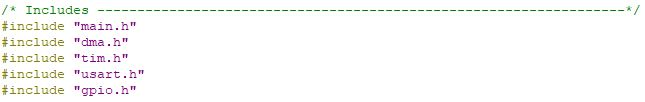
\includegraphics[width=\columnwidth]{./Images/Appendix/IMG_1.JPG}
	
	\vspace{0.5cm}
	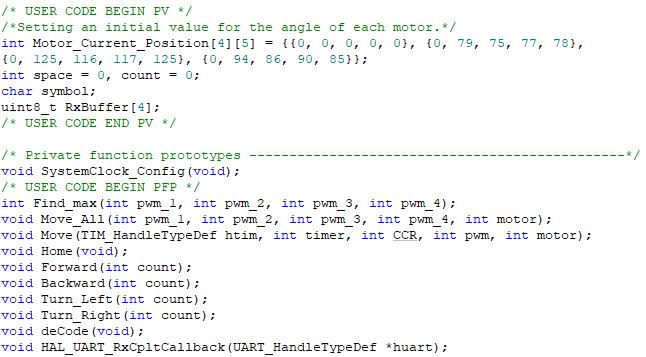
\includegraphics[width=\columnwidth]{./Images/Appendix/IMG_2.JPG}
	\end{figure}
	
	\begin{figure}[!h]
	\centering
	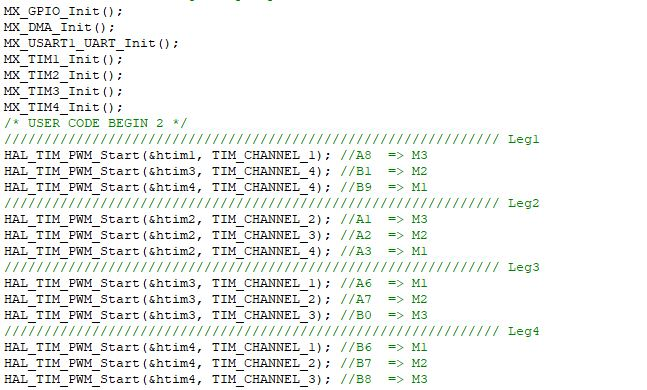
\includegraphics[width=\columnwidth]{./Images/Appendix/IMG_3.JPG}
		
	\vspace{0.5cm}
	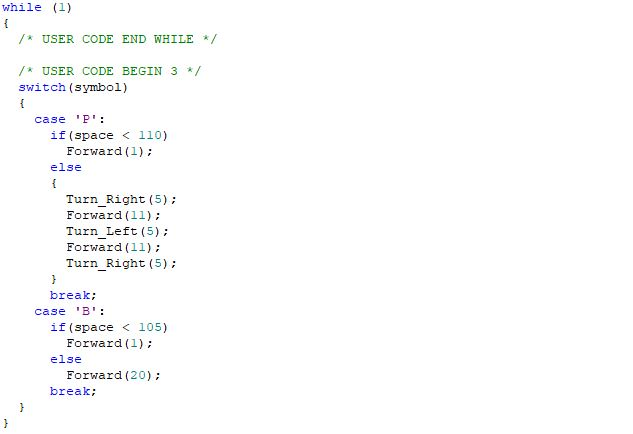
\includegraphics[width=\columnwidth]{./Images/Appendix/IMG_4.JPG}
	\end{figure}
	
	\begin{figure}[!h]
	\centering
	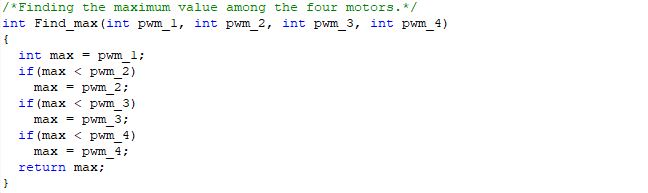
\includegraphics[width=\columnwidth]{./Images/Appendix/IMG_5.JPG}
		
	\vspace{0.5cm}
	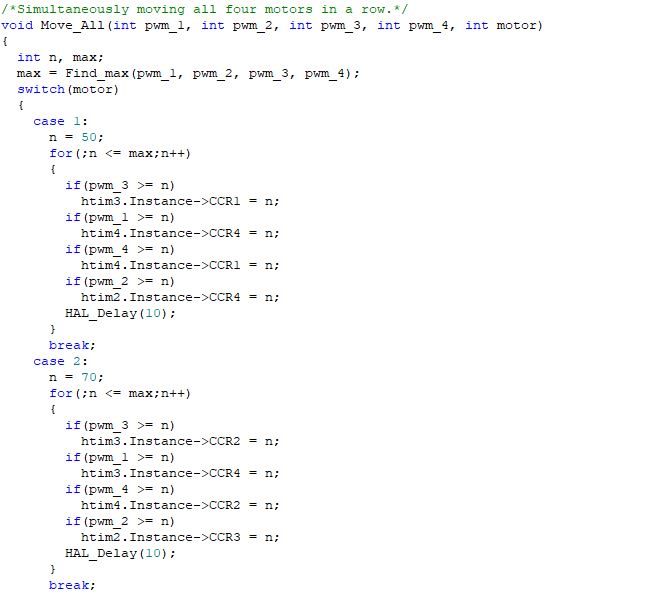
\includegraphics[width=\columnwidth]{./Images/Appendix/IMG_6.JPG}
	\end{figure}
	
	\begin{figure}[!h]
	\centering
	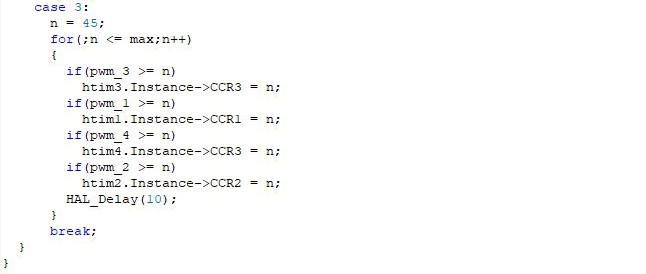
\includegraphics[width=\columnwidth]{./Images/Appendix/IMG_7.JPG}
	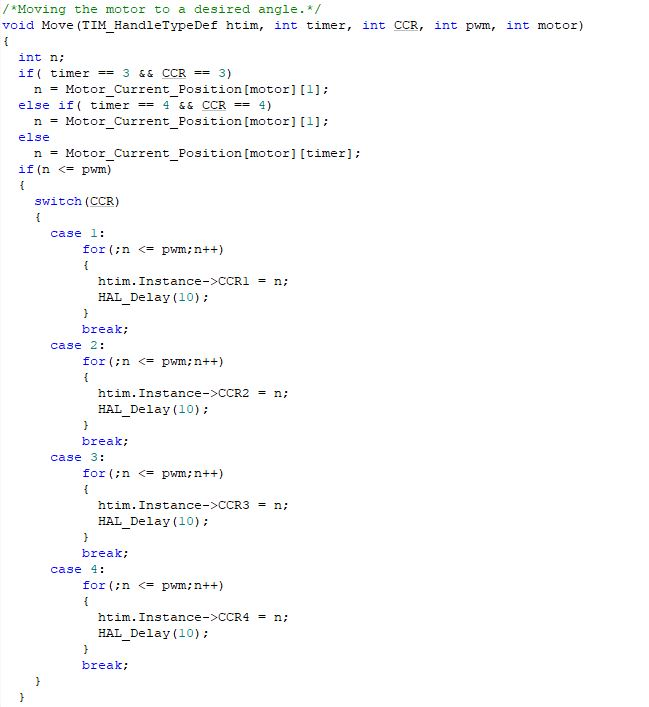
\includegraphics[width=\columnwidth]{./Images/Appendix/IMG_8.JPG}
	\end{figure}
	
	\begin{figure}[!h]
	\centering
	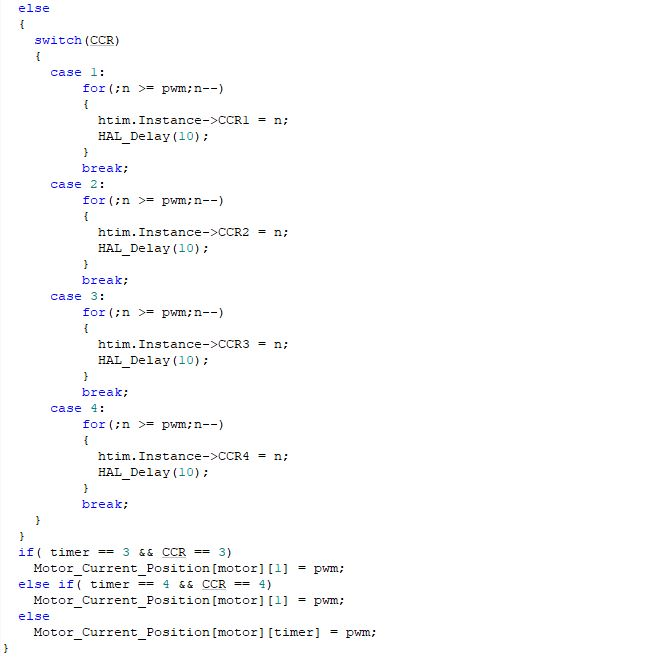
\includegraphics[width=\columnwidth]{./Images/Appendix/IMG_9.JPG}
			
	\vspace{0.5cm}
	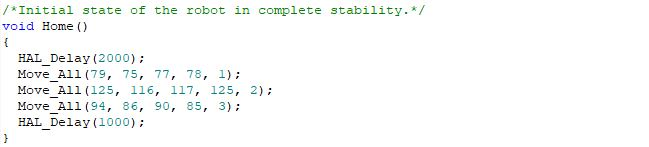
\includegraphics[width=\columnwidth]{./Images/Appendix/IMG_10.JPG}
	\end{figure}
	
	\begin{figure}[!h]
	\centering
	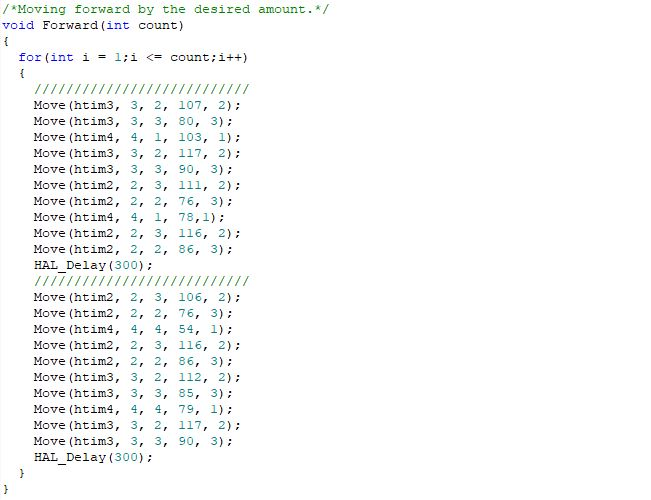
\includegraphics[width=\columnwidth]{./Images/Appendix/IMG_11.JPG}
		
	\vspace{0.5cm}
	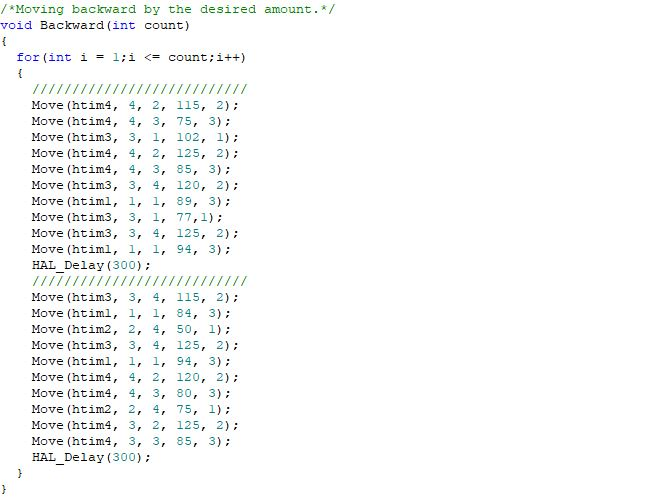
\includegraphics[width=\columnwidth]{./Images/Appendix/IMG_12.JPG}
	\end{figure}
	
	\begin{figure}[!h]
	\centering
	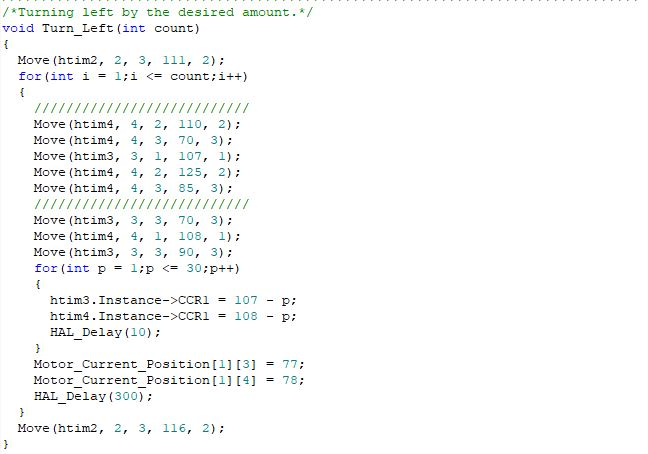
\includegraphics[width=\columnwidth]{./Images/Appendix/IMG_13.JPG}
	
	\vspace{0.5cm}
	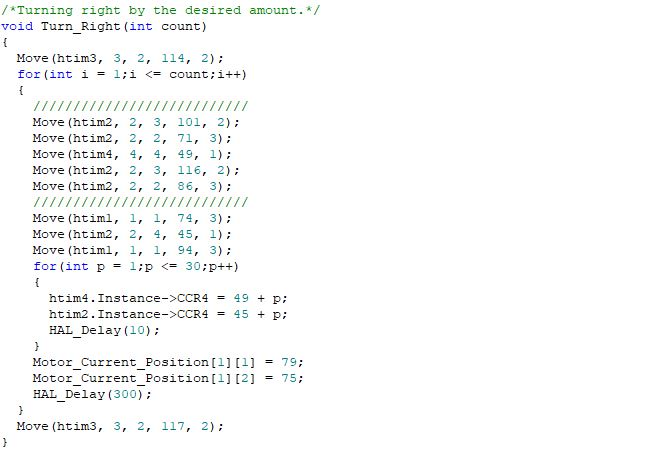
\includegraphics[width=\columnwidth]{./Images/Appendix/IMG_14.JPG}
	\end{figure}	
	
	\begin{figure}[!h]
	\centering
	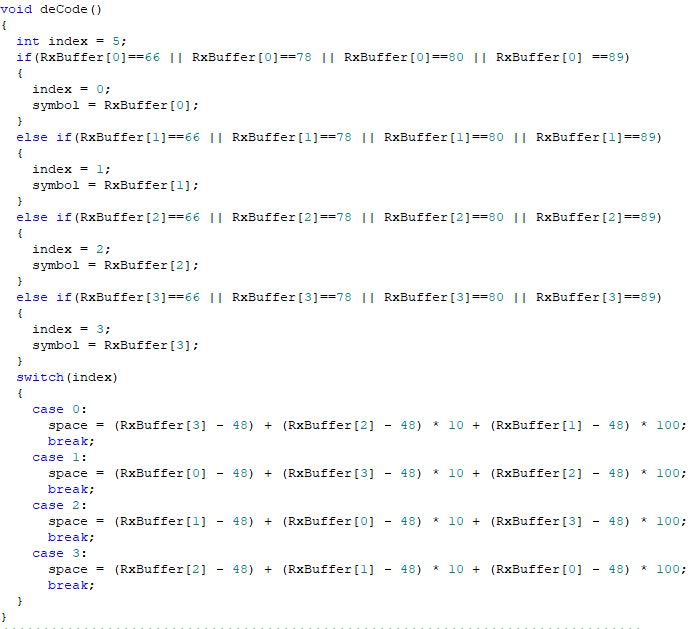
\includegraphics[width=\columnwidth]{./Images/Appendix/IMG_15.JPG}
	
	\vspace{0.5cm}
	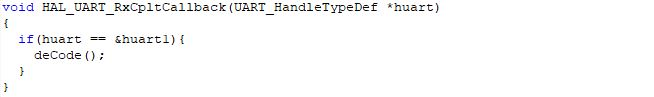
\includegraphics[width=\columnwidth]{./Images/Appendix/IMG_16.JPG}
	\end{figure}	
